\documentclass[8.5pt]{beamer}

\usepackage[utf8]{inputenc}
\usepackage[T5]{fontenc}
\usepackage{amsmath}
\usepackage{amssymb}
\usepackage{graphicx}
\usepackage{booktabs}

\setbeamersize{text margin left=2.5em, text margin right=2.5em}

\graphicspath{{./}{./assets/}{../../models/hasc/}}

\bibliographystyle{plain}

% ---------------------------------------------------------------
% Metadata
% ---------------------------------------------------------------
\title{Automatic Change-Point Detection\\in Time Series via Deep Learning}
\subtitle{A PyTorch Reimplementation and Extension of Li et al.\ \cite{li2024automatic}}
\author{
  Phạm Cung Lê Nhân Vũ \and
  Nguyễn Thị Thanh Hoài \and
  Nguyễn Nhật Quang
}
\institute{
  VNU-HCM University of Science\\
  Faculty of Mathematics and Informatics\\[4pt]
  \textit{Advisor: Tô Đức Khánh}
}
\date{April 2026}

% ---------------------------------------------------------------
\begin{document}
% ---------------------------------------------------------------

% --- Title slide -----------------------------------------------
\begin{frame}
  \titlepage
\end{frame}

% --- Outline ---------------------------------------------------
\begin{frame}{Outline}
  \tableofcontents[hideallsubsections]
\end{frame}

% ===============================================================
\section{Introduction}
% ===============================================================

\begin{frame}{Change-Point Detection}
  \begin{block}{Definition}
    Given a time series $X_1, X_2, \ldots, X_n$, identify points $\tau$ where
    the statistical properties (mean, variance, slope) change abruptly.
  \end{block}

  \bigskip
  \textbf{Two fundamental questions:}
  \begin{itemize}
    \item Does a change exist at all?
    \item If so, \emph{where} does it occur?
  \end{itemize}

  \bigskip
  \textbf{Real-world applications \cite{Truong_2020}:}
  \begin{itemize}
    \item Signal processing \& climate forecasting
    \item Cell biology (gene expression shifts)
    \item Human motion tracking (activity transitions)
    \item Financial market regime changes
  \end{itemize}
\end{frame}

\begin{frame}{Classical Approach: CUSUM and Its Limits}
  \textbf{Hypothesis test:}
  \[
    H_0: \mu_1 = \mu_2 = \cdots = \mu_n
    \qquad\text{vs.}\qquad
    H_1: \exists\,\tau \text{ s.t. } \mu_{\le\tau} \neq \mu_{>\tau}
  \]

  \textbf{CUSUM statistic \cite{page1954cusum}:}
  \[
    T_n = \max_{1\le k < n}\;\sqrt{\frac{k(n-k)}{n}}
             \left|\bar{X}_{1:k} - \bar{X}_{k+1:n}\right|
  \]
  Reject $H_0$ when $T_n > \lambda$; estimated change-point $\hat\tau = \arg\max$.

  \bigskip
  \textbf{Key limitations \cite{li2024automatic}:}
  \begin{itemize}
    \item Requires \textbf{i.i.d.\ Gaussian} noise — collapses to random guessing under
          auto-correlated or heavy-tailed distributions
    \item Manually designing optimal statistics for complex signals is impractical
  \end{itemize}
\end{frame}

% ===============================================================
\section{Theoretical Foundation}
% ===============================================================

\begin{frame}{Deep Neural Network Architectures}
  \begin{columns}[T]
    \begin{column}{0.48\textwidth}
      \textbf{Multi-Layer Perceptron (MLP) \cite{li2024automatic}}
      \begin{itemize}
        \item $L$ hidden layers, width $m_\ell$
        \item Input: sequence $X \in \mathbb{R}^n$
        \item Output: $\hat{Y} \in \{0,1\}$ (change / no change)
        \item Activation: shifted ReLU $\sigma_b$
      \end{itemize}
      \vspace{4pt}
      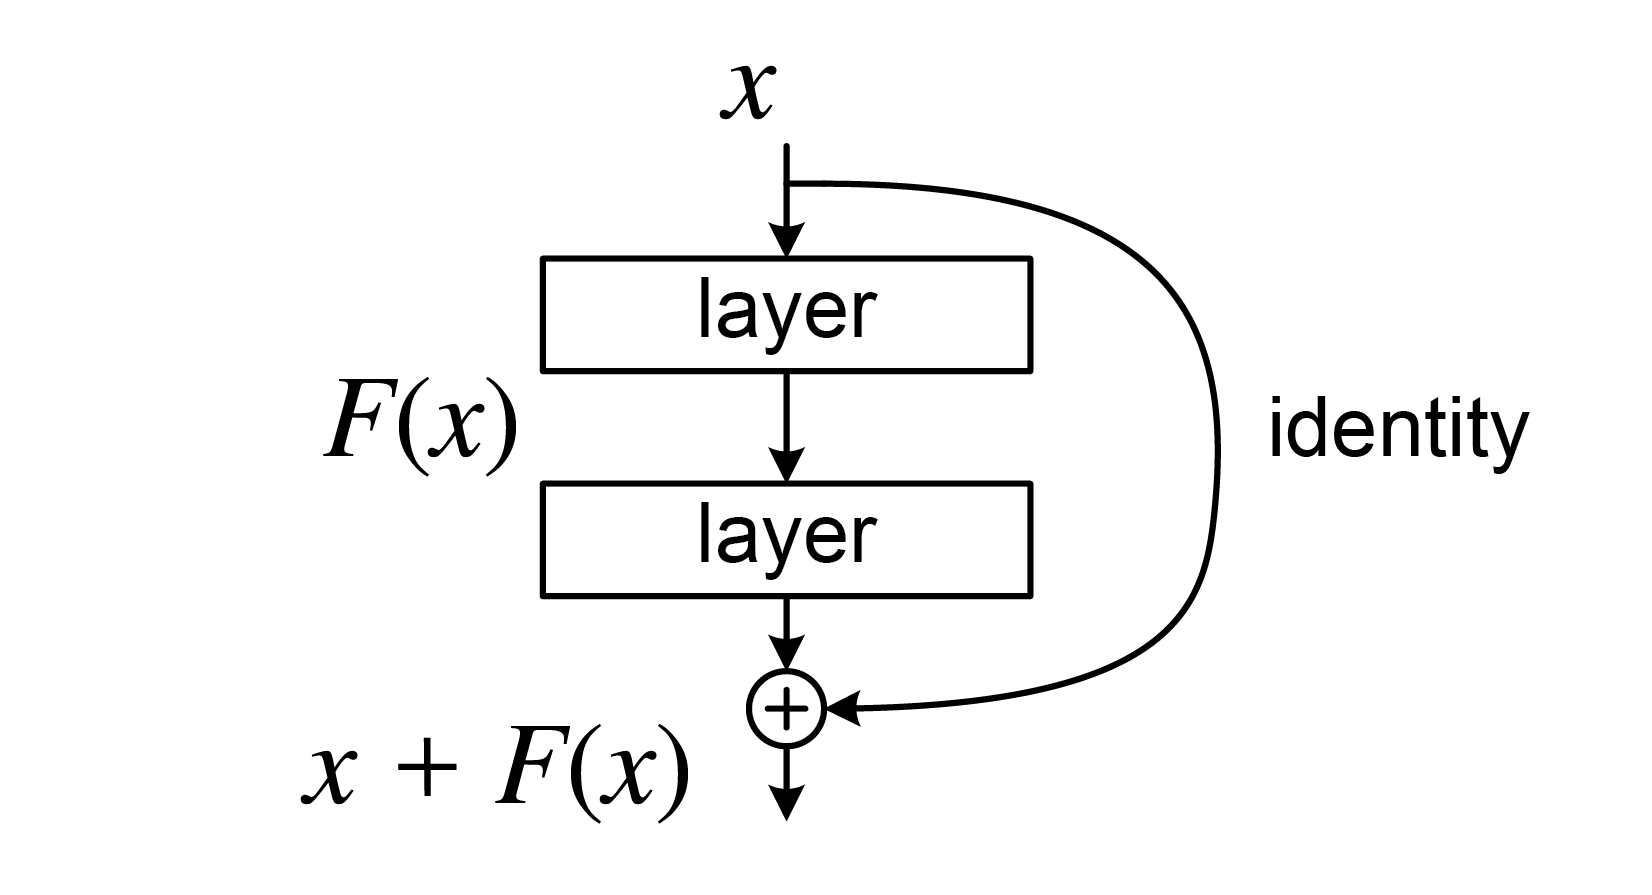
\includegraphics[width=\linewidth]{neural_network.png}
    \end{column}
    \begin{column}{0.48\textwidth}
      \textbf{Residual CNN (ResCNN) \cite{he2016resnet}}
      \begin{itemize}
        \item Skip connections prevent vanishing gradients
        \item Each block: $y = \mathcal{F}(x,\{W_i\}) + x$
        \item 21 residual blocks, base channels $= 32$
        \item Handles complex noise automatically
      \end{itemize}
      \vspace{4pt}
      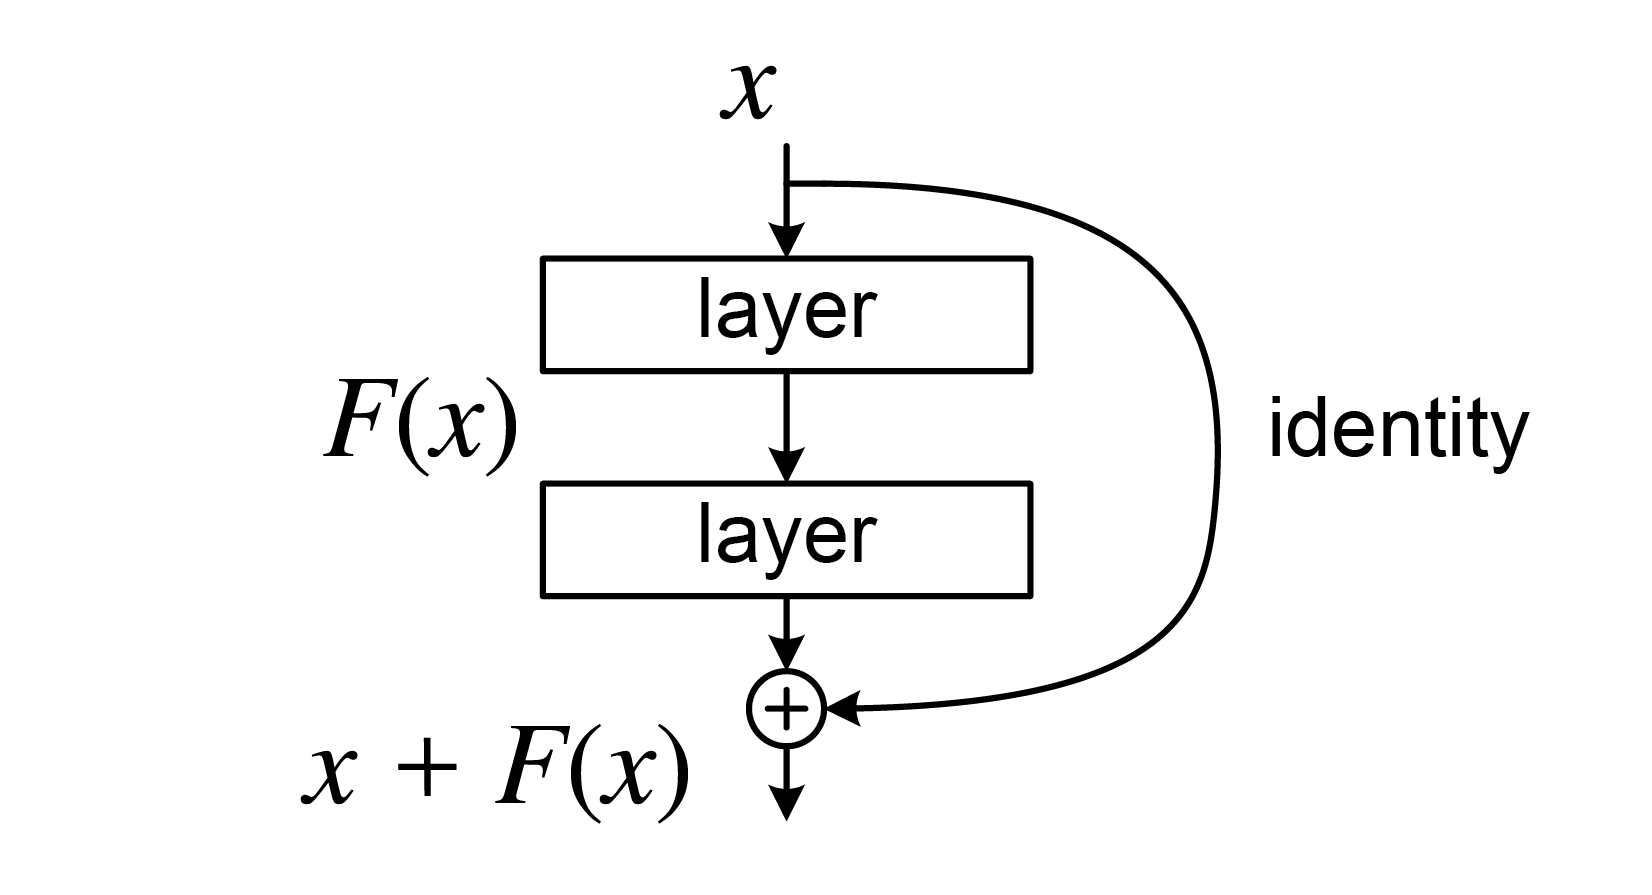
\includegraphics[width=\linewidth]{residual_block.png}
    \end{column}
  \end{columns}
\end{frame}

\begin{frame}{Notation for Theoretical Results}
  \begin{center}
  \begin{tabular}{@{}ll@{}}
    \toprule
    Symbol & Meaning \\
    \midrule
    $n$                    & Sequence length \\
    $B$                    & Minimum SNR parameter (defines class $\Theta(B)$); \\
                           & \quad actual signal $|\mu_L-\mu_R|\sqrt{\eta(1-\eta)} \ge B$,\; $\eta=\tau/n$ \\
    $N$                    & Training set size \\
    $\delta \in (0,1)$     & Confidence parameter (failure probability) \\
    $C$                    & Universal constant \\
    $L$                    & Number of hidden layers \\
    $h_{\text{ERM}}$       & Empirical risk minimiser (trained DNN) \\
    $\mathcal{R}(\cdot)$   & Misclassification risk $= P(h \neq Y)$ \\
    \bottomrule
  \end{tabular}
  \end{center}
\end{frame}

\begin{frame}{Key Theoretical Results \cite{li2024automatic}}
  \begin{block}{Theorem 1 — MLP $\equiv$ CUSUM}
    A single-hidden-layer MLP with \textbf{$2n-2$ ReLU units} can
    \emph{exactly represent} the CUSUM transformation.
    \[
      \mathcal{R}(h_{\text{ERM}}) \;\le\; n e^{-nB^2/8}
      + C\sqrt{\frac{n^2\log n\cdot\log N + \log(1/\delta)}{N}}
    \]
    Error $\to 0$ when $N \gg n^2\log n$.
  \end{block}

  \begin{block}{Theorem 2 — Pruned Deep MLP}
    An $L$-layer MLP with only $\mathbf{4\lfloor\log_2 n\rfloor}$ units per layer achieves:
    \[
      \mathcal{R}(h_{\text{ERM}}) \;\le\;
        2\lfloor\log_2 n\rfloor\, e^{-nB^2/24}
        + C\sqrt{\frac{L^2 n\log^2(Ln)\log N + \log(1/\delta)}{N}}
    \]
    Depth trades width for better generalization with fewer training samples.
  \end{block}
\end{frame}

% ===============================================================
\section{Methodology}
% ===============================================================

\begin{frame}{Problem Reformulation \cite{li2024automatic}}
  \textbf{Insight:} Convert hypothesis testing $\to$ binary classification.

  \[
    \psi: X \;\mapsto\; Y \in \{0, 1\}
    \quad
    \begin{cases} 0 & \text{no change point} \\ 1 & \text{change point present} \end{cases}
  \]

  \bigskip
  \textbf{Four synthetic noise scenarios (sequence length $n = 100$):}
  \begin{center}
  \begin{tabular}{@{}lll@{}}
    \toprule
    Scenario & Noise type & Challenge \\
    \midrule
    S1  & i.i.d.\ Gaussian $\mathcal{N}(0,1)$ & Baseline (CUSUM-friendly) \\
    S1' & AR(1), $\rho = 0.7$ & Fixed auto-correlation \\
    S2  & AR(1), $\rho_t \sim \text{Unif}[0,1]$ & Time-varying dependence \\
    S3  & Cauchy (heavy-tailed) & Infinite variance \\
    \bottomrule
  \end{tabular}
  \end{center}

  \bigskip
  \textbf{Data augmentation:} reverse each sequence to double training size.\\
  \textbf{Normalization:} min-max (S1/S1'/S2); trimmed robust (S3).
\end{frame}

\begin{frame}{Training Configuration}
  \textbf{Input:} raw sequence $x_t \in \mathbb{R}^n$ (canonical runs use no pre-transformations).
  Optional extensions — squared $x_t^2$ and cross-products $x_t\!\cdot\!x_{t+1}$ — are
  available in code but disabled in all reported experiments.

  \medskip
  \textbf{Loss:} Binary Cross-Entropy with logits
  \[
    \mathcal{L}_{\text{BCE}} = -\frac{1}{N}\sum_{i=1}^{N}
      \bigl[y_i\log\hat{y}_i + (1-y_i)\log(1-\hat{y}_i)\bigr]
  \]

  \medskip
  \begin{center}
  \begin{tabular}{@{}ll@{}}
    \toprule
    Hyperparameter & Value \\
    \midrule
    Optimizer & Adam \cite{kingma2015adam} ($\beta_1=0.9$, $\beta_2=0.999$) \\
    Learning rate & $0.001$ \\
    Epochs / Batch size & $200$ / $32$ \\
    Early stopping patience & $20$ epochs \\
    MLP width & $4\lfloor\log_2 n\rfloor$ units/layer \\
    ResCNN dropout & $0.3$ \\
    \bottomrule
  \end{tabular}
  \end{center}
\end{frame}

\begin{frame}{Multi-Change-Point Localization (Algorithm 1) \cite{li2024automatic}}
  Extends binary classifier to localize \emph{multiple} change points in long series.

  \bigskip
  \begin{enumerate}
    \item \textbf{Sliding window:} apply classifier to every window of size $n$
          along the full series
    \item \textbf{MOSUM-style smoothing:} compute rolling average of predicted
          probabilities $\bar{p}_t$
    \item \textbf{Segment detection:} identify maximal contiguous segments where
          $\bar{p}_t \ge \gamma$ (threshold $\gamma = 0.5$)
    \item \textbf{Localization:} within each segment, report
          $\hat\tau = \arg\max_t \bar{p}_t$ as the estimated change point
  \end{enumerate}

  \bigskip
  \begin{block}{Note on HASC}
    The main HASC result (Experiment 3) is \textbf{30-class activity classification},
    not localization. Algorithm 1 is an optional extension for binary change-point
    localization in longer sequences.
  \end{block}
\end{frame}

% ===============================================================
\section{Experiments \& Results}
% ===============================================================

\begin{frame}{Experiment 1: Single Change-Point on Synthetic Data}
  \textbf{Setup \cite{li2024automatic,autocpd2024}:} $n=100$,
  $N_{\text{train}}=10{,}000$ / $N_{\text{test}}=2{,}000$ (50/50 class balance),
  fixed splits with SHA-256 integrity hashes for reproducibility.

  \bigskip
  \begin{center}
  \begin{tabular}{@{}lcccc@{}}
    \toprule
    & \multicolumn{3}{c}{Detection Accuracy} & \\
    \cmidrule(lr){2-4}
    Scenario & MLP & ResCNN & CUSUM & Winner \\
    \midrule
    S1 (Gaussian)       & 0.9190 & \textbf{0.9255} & 0.8915 & ResCNN \\
    S1' (AR $\rho=0.7$) & 0.7290 & \textbf{0.7435} & 0.5005 & ResCNN \\
    S2 (AR time-vary)   & \textbf{0.7540} & 0.7525 & 0.5000 & MLP \\
    S3 (Cauchy)         & 0.5970 & \textbf{0.9475} & 0.5110 & ResCNN \\
    \bottomrule
  \end{tabular}
  \end{center}

  \bigskip
  \textbf{Key takeaways:}
  \begin{itemize}
    \item S1: all methods converge — confirms theory
    \item S1'/S2: CUSUM $\approx$ random guessing; DNNs maintain $>72\%$
    \item S3: ResCNN \textbf{+44 pp} over CUSUM — strongest result
  \end{itemize}
\end{frame}

\begin{frame}{Experiment 3: Real-World HASC Dataset \cite{hasc2011}}
  \textbf{Task:} Classify 7-second accelerometer windows into 30 activity states
  (6 pure + 24 transition activities).

  \bigskip
  \begin{columns}[T]
    \begin{column}{0.48\textwidth}
      \textbf{Setup}
      \begin{itemize}
        \item Window size: $n = 700$ samples
        \item 3-axis input (ResCNN multi-channel)
        \item Training: 13\,380 windows, persons 101–105\textsuperscript{*}
        \item 30-class softmax output
      \end{itemize}
    \end{column}
    \begin{column}{0.48\textwidth}
      \textbf{Results (best at epoch 121)}
      \begin{itemize}
        \item Val.\ loss: $0.1749$
        \item Val.\ accuracy: $\mathbf{96.21\%}$
        \item Macro F1: $0.9042$
        \item Weighted F1: $0.9608$
      \end{itemize}
    \end{column}
  \end{columns}

  \medskip
  {\scriptsize *Reported checkpoint provenance; current split metadata may reflect later reruns.}

  \medskip
  \begin{block}{Key finding}
    The same ResCNN architecture used for binary synthetic classification scales
    directly to 30-class real-world sensor data with no architectural redesign.
  \end{block}
\end{frame}

\begin{frame}{HASC Training Dynamics \& Confusion Matrix}
  \begin{columns}[T]
    \begin{column}{0.50\textwidth}
      \centering
      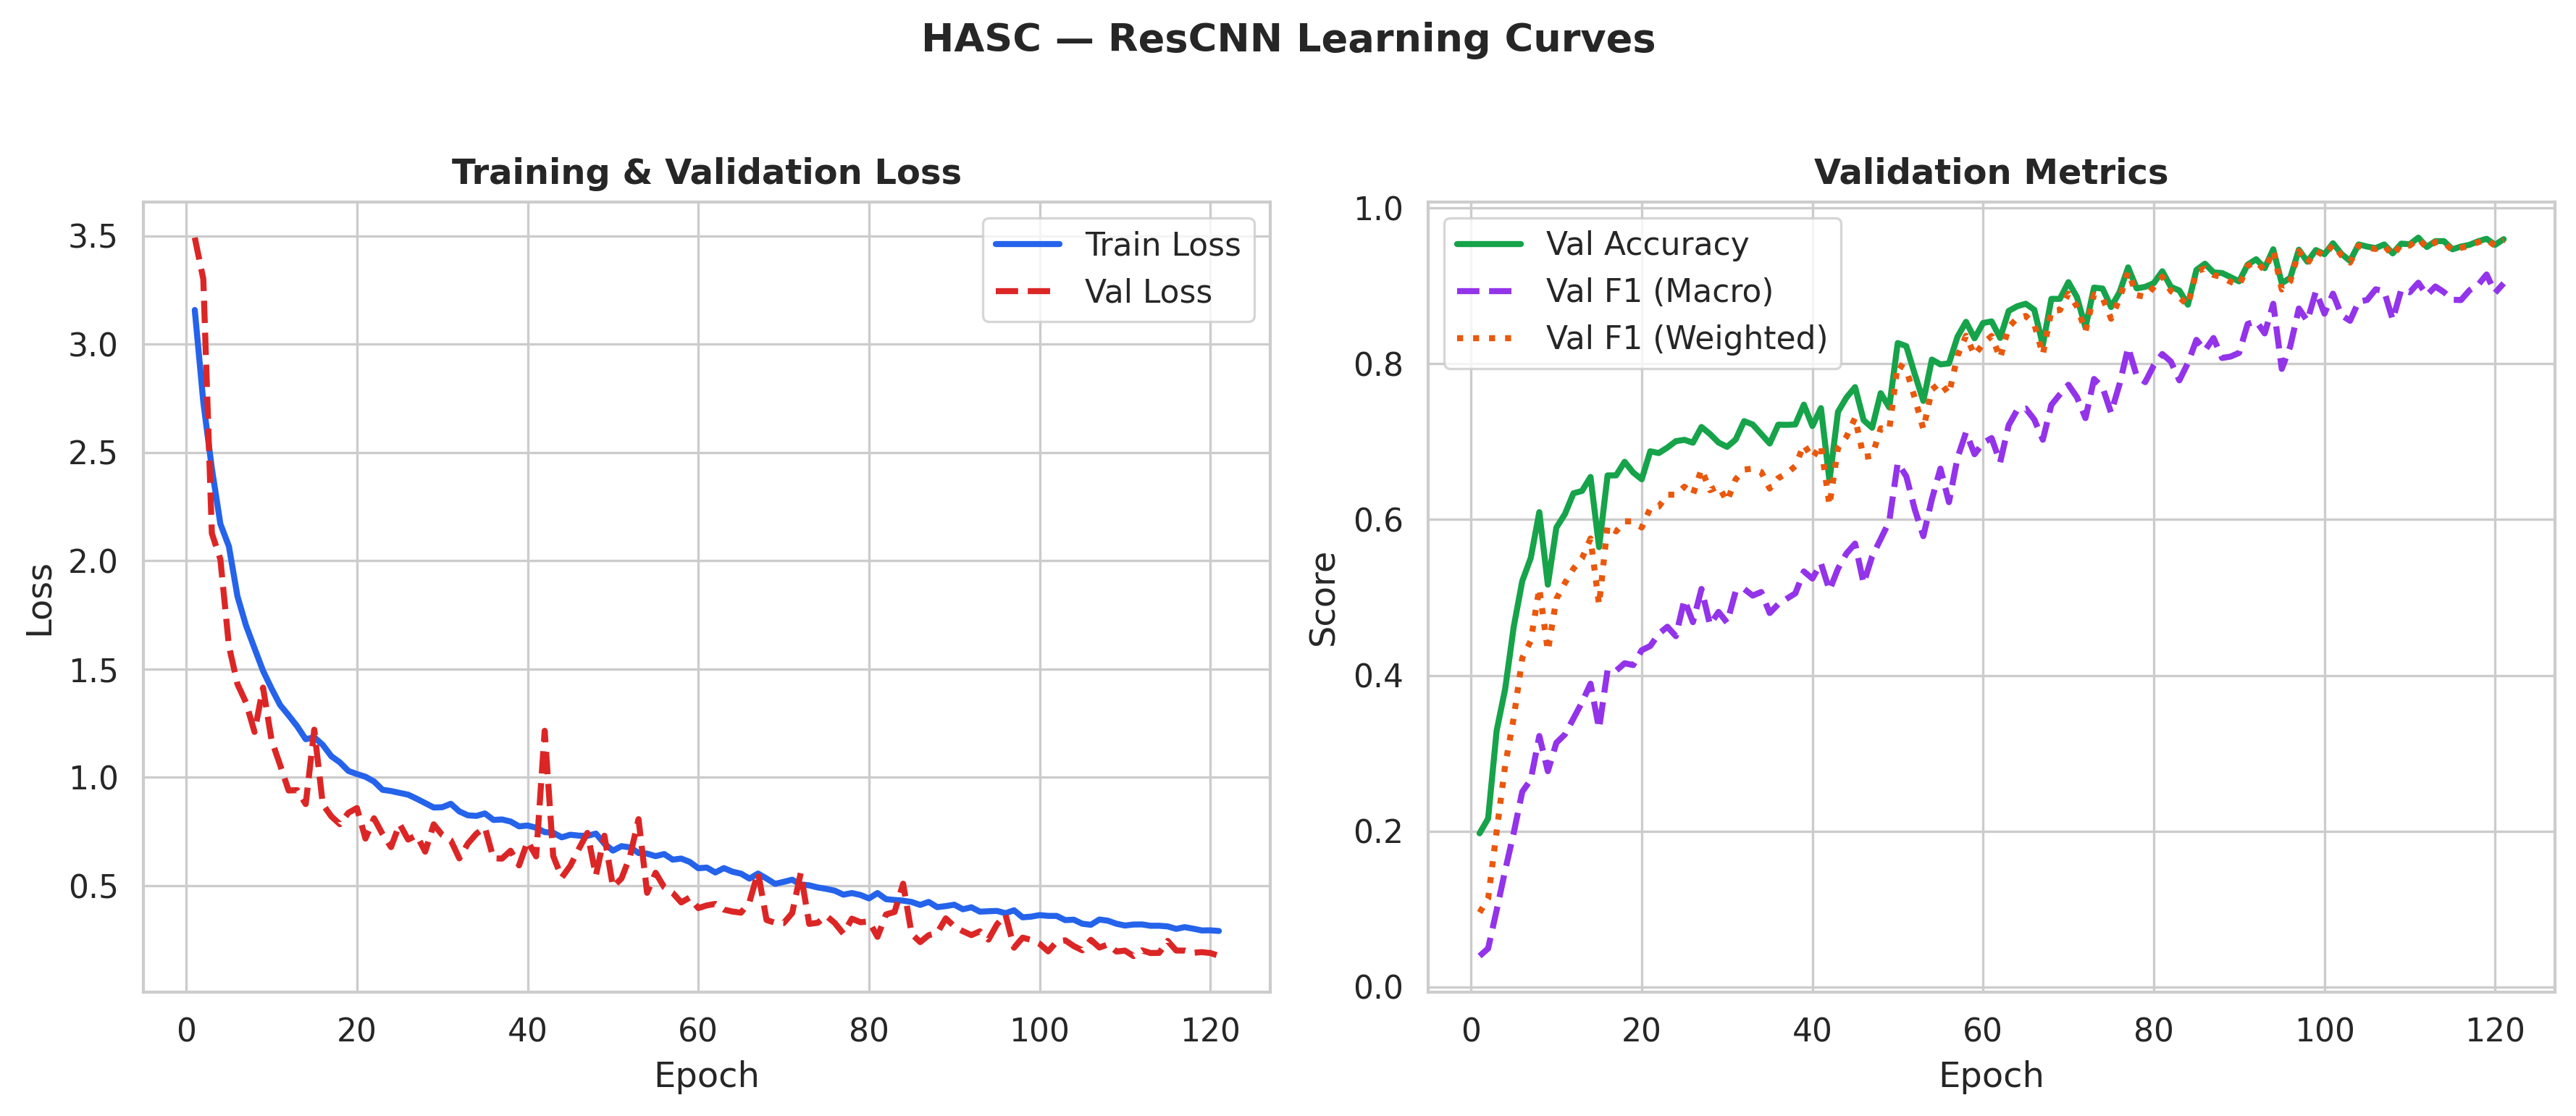
\includegraphics[width=\linewidth]{hasc_learning_curve.png}\\
      \small Fast convergence; stable val.\ loss after $\sim$50 epochs;\\
      F1 $> 0.90$ consistently.
    \end{column}
    \begin{column}{0.48\textwidth}
      \centering
      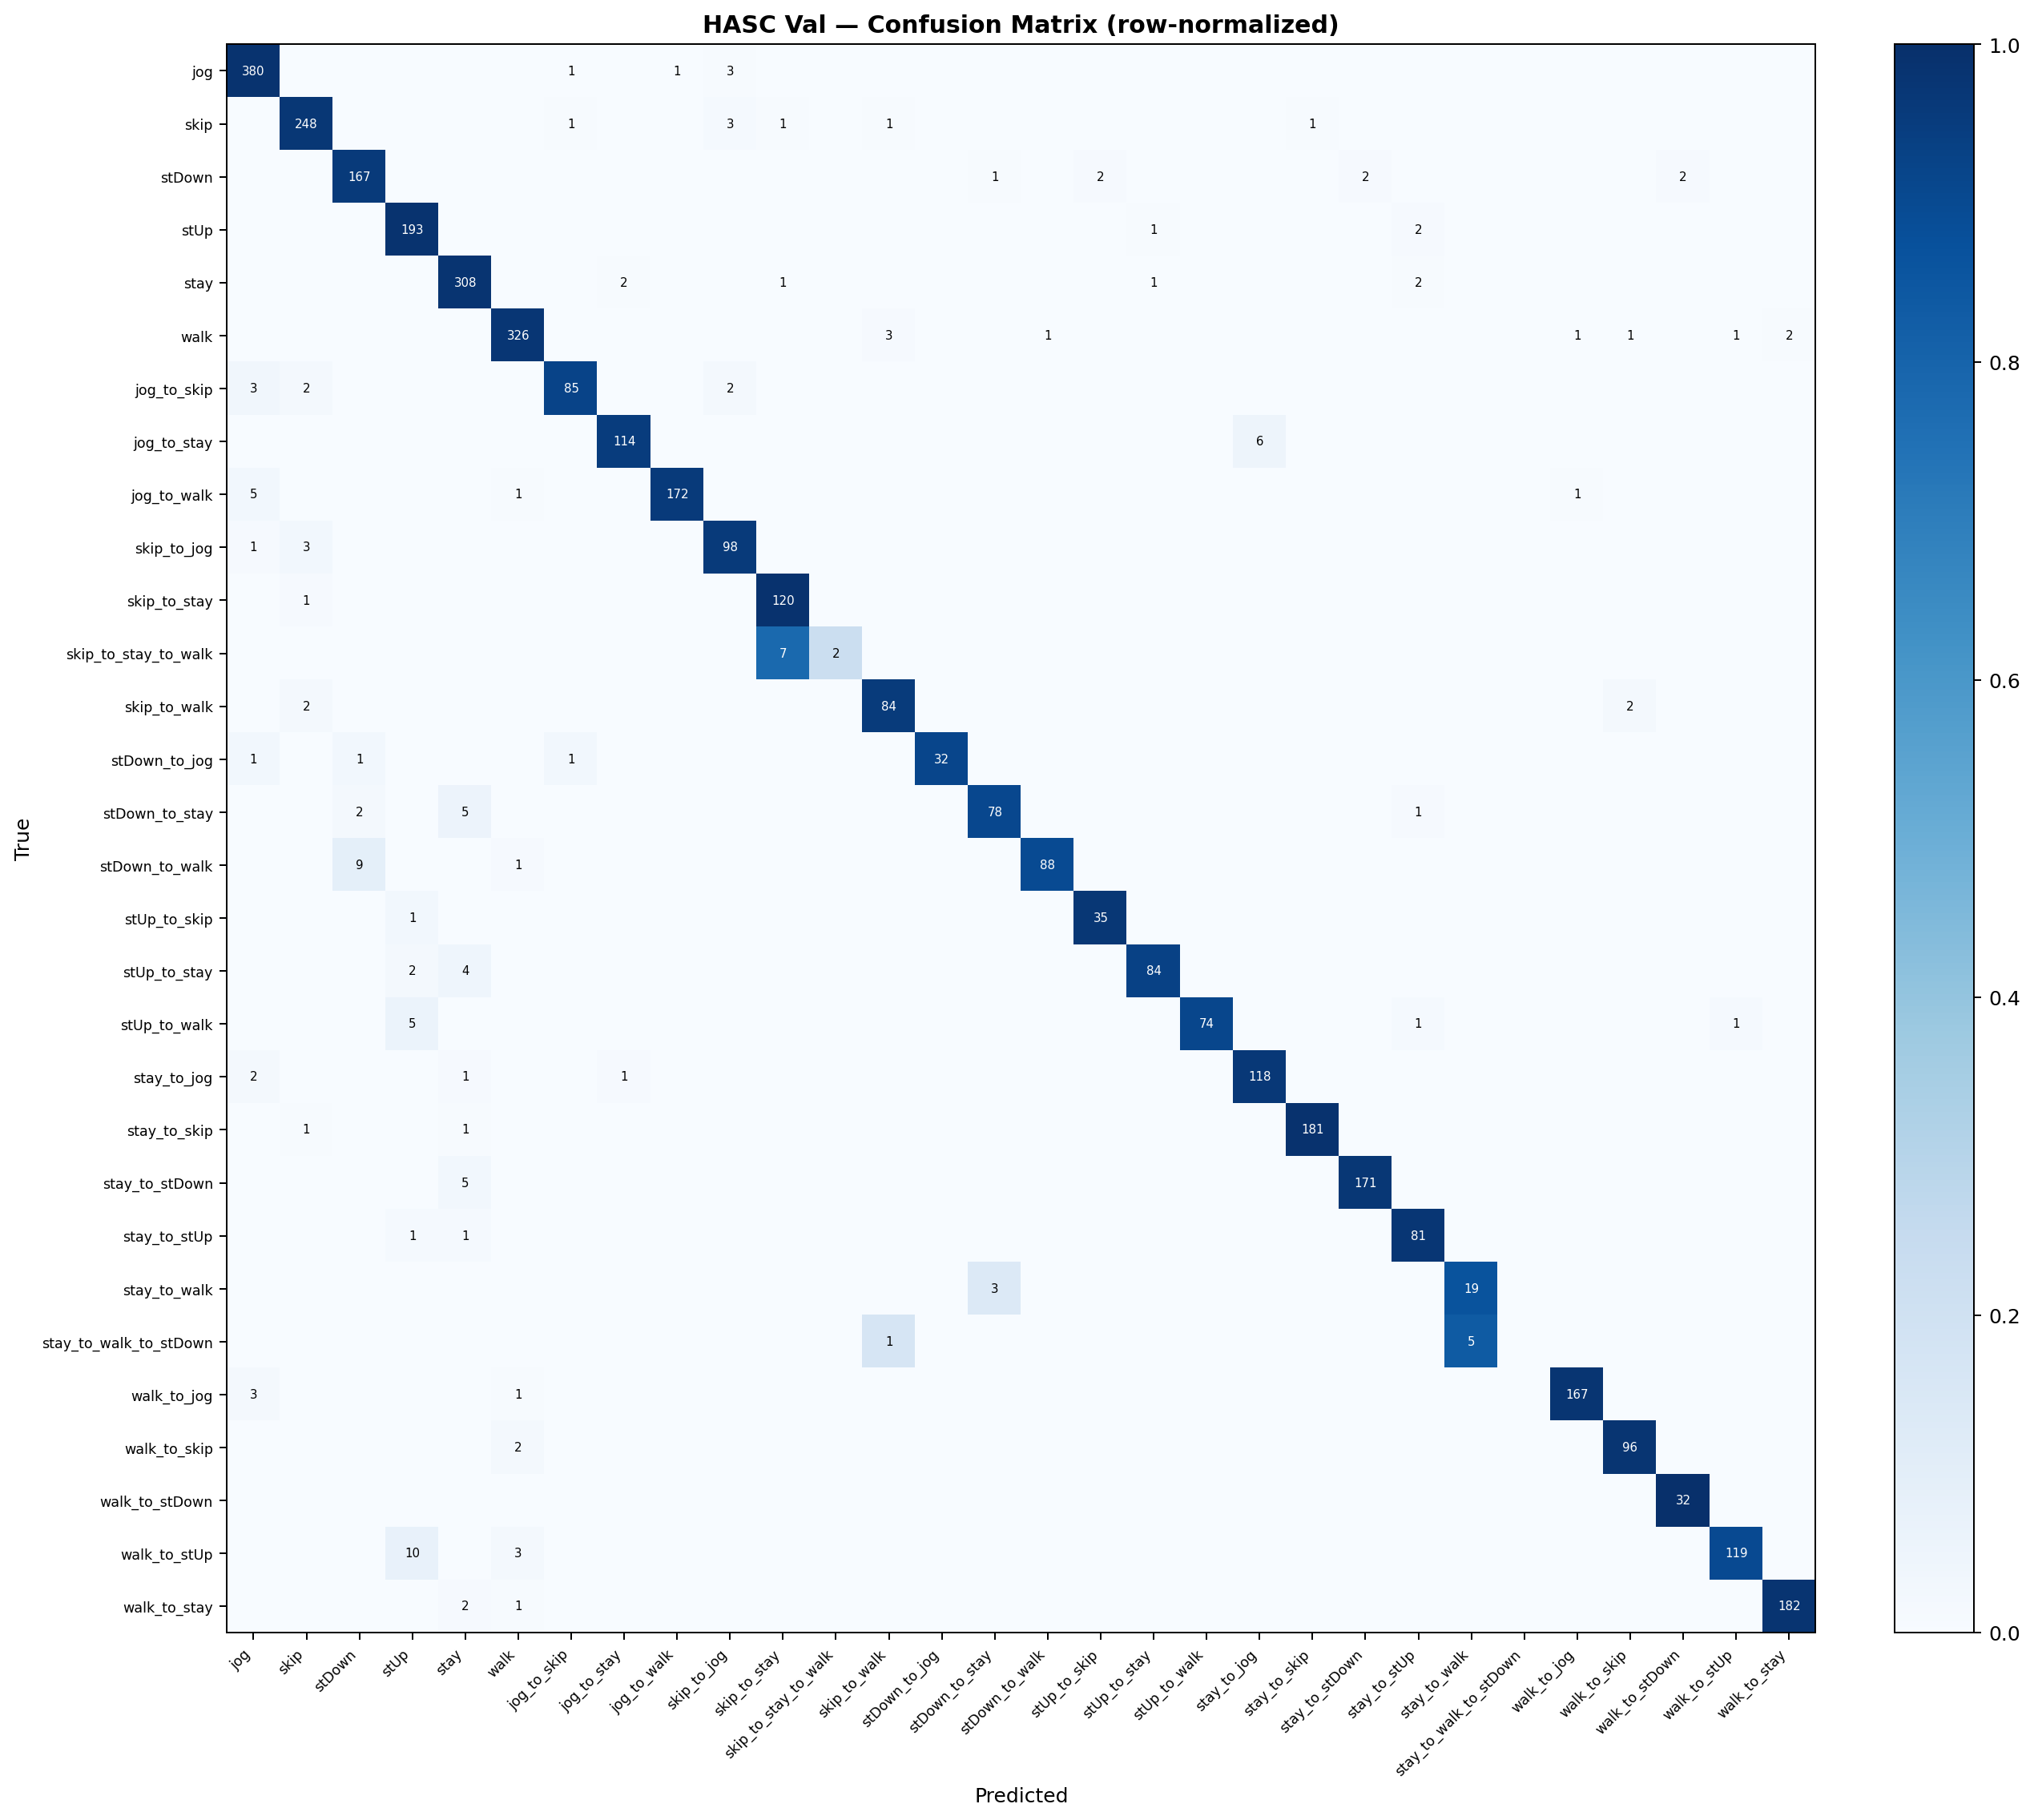
\includegraphics[width=\linewidth]{hasc_confusion.png}\\
      \small 30$\times$30 confusion matrix (4006 val.\ samples).\\
      Most classes: near-perfect recall.\\
      Rare transitions ($<$10 samples) show lower recall.
    \end{column}
  \end{columns}
\end{frame}

% ===============================================================
\section{Conclusion}
% ===============================================================

\begin{frame}{Conclusion — Contributions}
  \begin{itemize}
    \setlength\itemsep{8pt}
    \item \textbf{Reproducible PyTorch reimplementation} of \cite{li2024automatic}
          with deterministic synthetic datasets and SHA-256 integrity checks
    \item \textbf{Validated theory–practice alignment:} MLP/ResCNN match CUSUM
          on Gaussian data and substantially outperform on complex noise
          (up to $+44$ pp on Cauchy distributions)
    \item \textbf{Real-world scaling:} same ResCNN achieves \textbf{96.21\%}
          accuracy on 30-class HASC \cite{hasc2011} activity recognition
  \end{itemize}

  \bigskip
  \begin{center}
    \large\textit{Deep learning is not just a substitute for classical statistics —}\\
    \textit{it adapts where classical methods break down.}
  \end{center}
\end{frame}

\begin{frame}{Limitations \& Future Work}
  \begin{itemize}
    \setlength\itemsep{10pt}
    \item \textbf{Multi-CP localization} (Algorithm 1) demonstrated qualitatively only —
          quantified $|\hat\tau - \tau|$ error over many sequences is needed
    \item \textbf{Limited baselines:} only CUSUM \cite{page1954cusum} compared;
          non-parametric and robust methods (e.g.\ PELT, E-divisive) should be added
    \item \textbf{No ablation studies} on pre-transformations, robust normalization,
          or ResCNN depth; HASC evaluation needs person-held-out splits
  \end{itemize}
\end{frame}

% ===============================================================
\begin{frame}[allowframebreaks]{References}
  \bibliography{bibliography}
\end{frame}

\begin{frame}
  \begin{center}
    \Huge Thank You\\[16pt]
    \large Questions?\\[24pt]
    \normalsize
    \begin{tabular}{rl}
      Code:    & \texttt{github.com/ngnquanq/change\_point\_detection}
    \end{tabular}
  \end{center}
\end{frame}

\end{document}
